%!TEX root = ../username.tex
\chapter{Introduction} \label{sec:introduction}

% \hl{Why should one care about this paper} 
When comparing the human brain with the machine, we can see that humans excel at interpreting data on a high level and in a more abstract format. In contrast, the machine has higher computational power when it comes to raw numerical data. Additionally, by Moore's law, the number of transistors in a dense integrated circuit doubles every two years, which is associated with the computational power of machines becoming more and more powerful. Therefore, it is reasonable to believe that if a machine can interpret and understand the representation of objects beyond raw numerical data, then the machine can process and react much faster than humans. In other words, vision in machines proves to be very beneficial to humans when it comes to situations requiring quick reactions. Such situations can be seen or encountered every day through traffic. If done correctly, the machine with vision can predict and avoid traffic accidents faster than humans. Thus, the machine can help create a safer traffic flow.

%% https://www.tesla.com/blog/your-autopilot-has-arrived %
%% https://www.nbcnews.com/business/autos/driverless-tesla-will-travel-l-nyc-2017-says-musk-n670206 
Over the last decade, we have seen multiple raised startups, as well as big corporations, pour millions of dollars into research to try to obtain a piece of the autonomous vehicle market which is valued at billions of dollars. One of the leading companies in the field of the autonomous vehicle is Tesla. In October 2015, Tesla released the Tesla Version 7.0 software enabling the Autopilot feature for the Model S, and promised that the car would be fully autonomous in 2017. However, in July 2022, 2 different Tesla cars crashed while on autopilot, and each crash caused the death of a motorcyclist. Additionally, in 2019, a Tesla autopilot crashed into a Honda Civic and killed two people. Not to mention, there are 273 Tesla crashes involving the autopilot system reported just in 2019. As we can see, as of 2022, we have yet to be able to develop a fully autonomous system.

To be able to achieve a fully autonomous vehicle, it is crucial to identify which module or modules in the autonomous driving modular pipeline are at fault. The autonomous driving modular pipeline consists of four components. These components are Perception and Localization, High-Level Path Planning, Behavior Arbitration, and Motion Controllers [\ref{fig:autonomous_driving_pipeline}].

\begin{figure}[!ht] \centering
    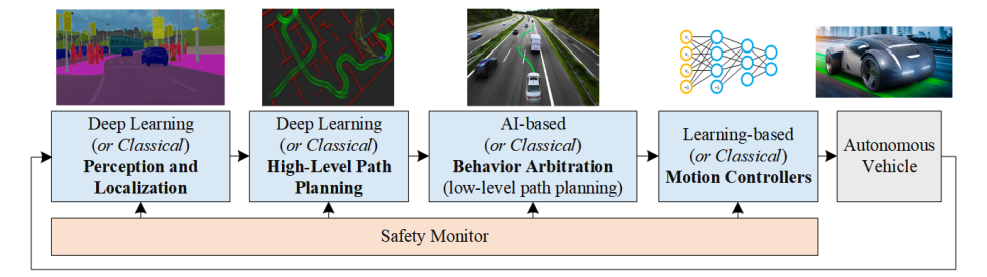
\includegraphics[keepaspectratio=true,width=6in]{figures/autonomous_driving_modular_pipeline.png}
    \caption{Deep Learning Based Autonomous Driving Modular Pipeline \cite{grigorescu_trasnea_cocias_macesanu_2020}}
    \label{fig:autonomous_driving_pipeline}
\end{figure}

To identify which module or modules are at fault, we need to understand and analyze each module of the modular pipeline. In this paper, we will only look at Perception and Localization, the first module in the autonomous vehicle pipeline. The Perception and Localization module is responsible for answering two questions: "Where is the car?" and "What is around the car?" \cite{liu_2020}. To perform this function, the module needs to utilize the sensing hardware and the software to understand the scene. Such hardware can be LiDAR, cameras, or other sensors. Nonetheless, they are all used for getting the information surround the vehicle and feeding those data to the software functionality of the module.

Getting the information surround the vehicle is straightforward as it simply records and passes those recorded data to the software functionality. However, understanding the scene is a more challenging task and not as straightforward. Unlike human beings, the machine sees and processes objects differently from our eyes and brain. While we see the object as a whole, the machine sees it as a grid of values that do not have any connection with one another. For this reason, the Computer Vision field tackles this problem and tries to create algorithms that are able to make sense of the object representation beyond the raw numerical data. The most important groups of algorithms in the Computer Vision field for understanding traffic scenes are video segmentation algorithms.

There are two types of video segmentation exist. The two are video semantic segmentation and video instance segmentation. In the video semantic segmentation algorithm, for each scene, objects in the scene are grouped and classified based on categories. On the other hand, video instance segmentation detects each instance of each category for each scene. Comparing semantic segmentation and instance segmentation, we can see that instance segmentation proposes a higher accuracy as it is able to see each instance of a class. That is, the instance segmentation algorithm will be able to distinguish between a car, a truck, and a bicycle if present instead of just vehicles class like semantic segmentation.

Since video instance segmentation algorithms give higher detection accuracy, in this paper, we will assume an algorithm from this group will be used for the Perception and Localization module. Knowing a video is a sequence of images, many video instance segmentation algorithms were proposed based on an algorithm in image instance segmentation. One example of such an algorithm is MaskTrack R-CNN which includes a new tracking branch to the well-known image instance segmentation Mask R-CNN. For that reason, to understand video instance segmentation, we first need to understand and analyze image instance segmentation. More specifically, this paper will discuss the building block of image instance segmentation algorithms. We then analyze and compare the performance of two well-known image instance segmentation algorithms, the Mask R-CNN and You Only Look Once version 7 (YOLOv7). Furthermore, we will want to identify if misidentified by these image instance segmentation algorithms causes the autonomous driving pipeline to fail and result in accidents.
